\chapter{Simulator description}
\label{chap:description}

{\it GridSim}\footnote{
{\it GridSim} is released under GPLv3.0.
It can be downloaded from: \href{https://github.com/Robolabo/gridSim.git}{https://github.com/Robolabo/gridSim.git} 
} is an open source simulator developed to analyze the power balances on a virtual electrical grid.
Figure~\ref{fig:gridsim_sch} shows a scheme of its modular architecture.
The grid is composed by lines.
A line represents a set of nodes with the same features.
The nodes are complex elements connected to the lines which can be equipped with different types of consumption, {\it Distributed Energy Resources} (DER) technologies and control systems.
These nodes can represent from a single device which only consumes as a single device to a complex microgrid.
In addition, a base consumption function can be added to the grid.
It represents an uncontrollable consumption which is added to the aggregated consumption of the simulated grid.

The structure of a grid is defined by an XML file.
In this file, the number of lines and the number of nodes per line can be defined.
Each line has a concrete type of node; 
it means that all the nodes of each line have the same features.
{\it GridSim} can run multiple executions in parallel.
This feature of the simulator has been implemented by making use of the MPI\footnote{
Message Passing Interface (MPI) is a standardized and portable message-passing system designed by a group of researchers from academia and industry to function on a wide variety of parallel computers.
The standard defines the syntax and semantics of a core of library routines useful to a wide range of users writing portable message-passing programs in different computer programming languages.
} protocol.
\begin{figure}[!t]	
	\begin{center}
		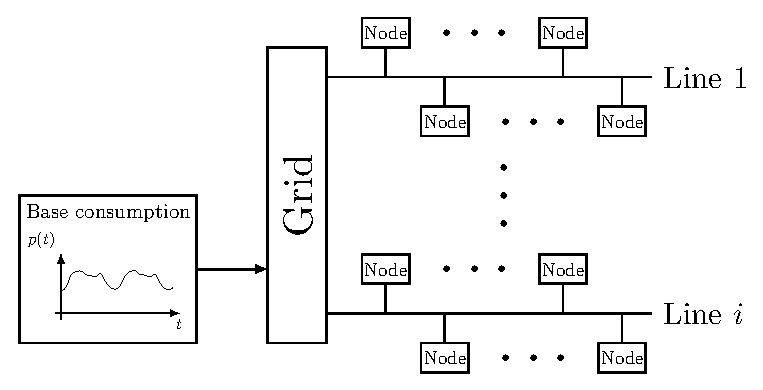
\includegraphics[width=0.9\textwidth]{gridsim_sch.eps} \\ 
		\caption[Scheme of the modular architecture of {\it GridSim} simulator.]
		{Scheme of the modular architecture of {\it GridSim} simulator.}		
		\label{fig:gridsim_sch}	
	\end{center}
\end{figure}

{\it GridSim} calculates the power balances of every node and they are aggregated in their common line.
The aggregated consumption of the virtual electrical grid is calculated as the sum of the power balances of every line plus the base consumption function.
The nodes can be equipped with different controllers to control the possible elements which a node is composed of.
For example, the charge power of the storage system can be controlled by a battery controller. %as the presented in Section~\ref{sec:bat_ctr}.
The controllers can obtain information from every element of the {\it GridSim} simulator.
%SG algorithm has been implemented in these nodes.
%The algorithm receives information from the grid about the aggregated consumption and the local node.
%It uses this information to schedule the deferrable load, indicating every deferrable load the activation time.

Algorithm~\ref{alg:gridsim} describes the operation of {\it GridSim}.
In the first place, the simulator is initialized---see from line $1$ to $3$ .
The virtual electrical grid is created by using a configuration file which indicates structure of the grid.
In addition, the counter of {\it time steps} is set to zero.
A time step is one execution of the main loop of the simulator.
It is the virtual clock of a simulation which marks the events that happen.
A time step is related to an amount of time in the real world.
For example, if a time step represents one minute, 
in each execution of the main loop, the power balances are calculated for one minute in the real world.
The lower the amount of time in the real world is, the higher the accuracy of the simulator is, but also the greater the computing power. 
After {\it GridSim} is initialized, the main loop begins.
The main loop simulates the virtual electrical grid, the virtual users and controllers in each time step.
The counter of time steps is increased at the end of this loop.
When the main loop finishes, the simulation finishes.
This condition is satisfied when the counter of time steps reaches a certain value indicated in the configuration file---see the condition of line $5$.
\begin{algorithm}[!t]
\caption[Main loop of {\it GridSim} simulator.]{High-level description of the main loop of {\it GridSim} simulator.}\label{alg:gridsim}
\begin{algorithmic}[1]
\State $\text{/* Initialization */}$
\State $\text{createGrid($<configurationFile>$)}$ 
\State $TimeStep \gets 0$
\State $\text{/* Main Loop */}$
\While{ $TimeStep < TimeStepLimit$ } 
	\State $\text{/* Execute main control function */}$
	\State $\text{mainControlFunction()}$ 
	\State $\text{/* Execute virtual user functions on all nodes */}$
	\For{$i<numNodes$}
		\State $\text{node[i]$\rightarrow$userFunction()}$
	\EndFor
	\State $\text{/* Execute control functions on all nodes */}$
	\For{$i<numNodes$}
		\State $\text{node[i]$\rightarrow$controlFunction()}$
	\EndFor
	\State $\text{/* Execute grid energy balance - physics engine */}$
	\State $\text{gridExecutionFunction()}$
	\State $TimeStep++$
\EndWhile
\end{algorithmic}
\end{algorithm}
